\documentclass[11pt]{article}

\usepackage{sectsty}
\usepackage{graphicx}
\usepackage[T1]{fontenc}
\usepackage[utf8]{inputenc}
\usepackage[a4paper, total={6in, 10in}]{geometry}
\usepackage{mathdots}%
\usepackage{amsmath}
\usepackage{amssymb}
\usepackage{hyperref}
\usepackage{caption}

% \setcitestyle{open={},close={}}

% \renewcommand{\figurename}{Obrázek}
\captionsetup[figure]{font={rm,small},labelfont=bf}


\title{ Informatics and Cognitive Science 2 - Final project}
\author{ David Beinhauer }
\date{\today}

\begin{document}
\maketitle



\section{Intoduction}
Parkinson's disease (PD) is a brain disorded, characterized by a motor and cognitive
disfunctions, caused by dopamine depletion in the basal ganglia. A distinctive feature of
PD is associated with slow oscillations and increased synchrony of neural activity 
in basal ganglia. It has been shown that strength of inhibitory inputs from globus 
pallidus external (GPe) is a key parameter in controling the oscillations. Furthermore,
deep brain stimulation (DBS) of the neurons from subthalamic nucleus (STN) can lead to 
quenching of oscillations in both populations of neurons (GPe and STN). Goal of this 
project is to create simplified model of the neural network inspired by the paper of 
Kumar et al. and try to replicate the results from the paper.



\section{Model Description}
We use NEST simulator to model and simulate our network. The network consists of 
2 populations of neurons. Inhibitory neurons from GPe and excitatory neurons from STN. 
These neurons are connected both within and across the populations. Nevertheless,
all neurons recieve external excitatory input from outside (to simulate input from 
cortex). More complex explanation of the network could be seen in the project description.

The whole simulation runs for 3000 ms. First stage of the simulation should represent the
healthy state. In order to simulate the dopamine depleted state (PD), 
we increase the inhibitory input to GPe using Poisson generator at time 1000 ms.
At time 2000 ms we simulate the DBS using direct current generator to STN population.



\section{Results}

\begin{figure}[tb]
    \centering
    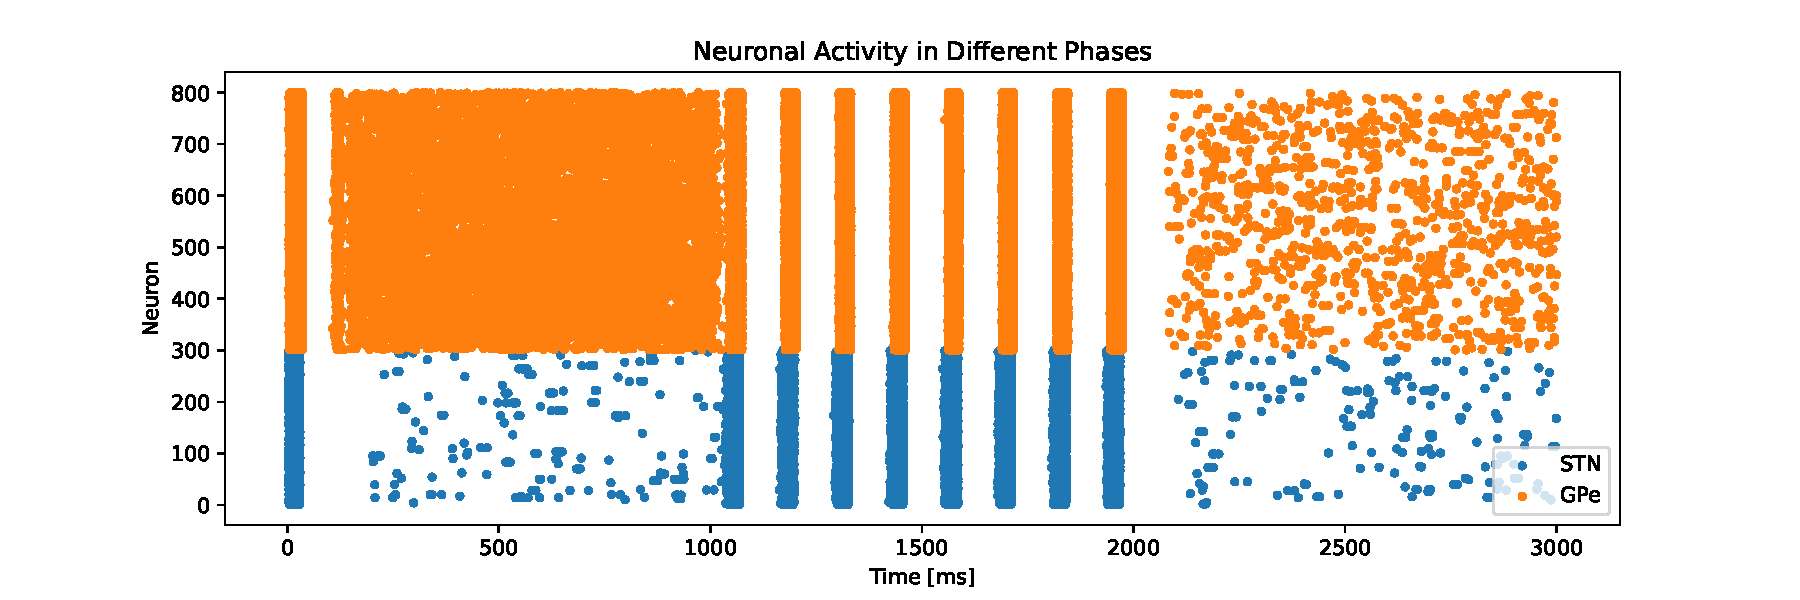
\includegraphics[width=\textwidth]{images/raster_spikes.pdf}
    \caption{\textbf{Neuronal activity in different phases:} 
    Raster plot of neuronal activity in time in 3 different phases of 
    simulation. Time 0-1000 ms no additional input, time 1000-2000 ms additional 
    inhibitory Poisson input to GPe, time 2000-3000 ms additional Poisson input 
    to GPe and DBS to STN.}
    \label{fig:raster_plot}
\end{figure}

\begin{figure}[tb]
    \centering
    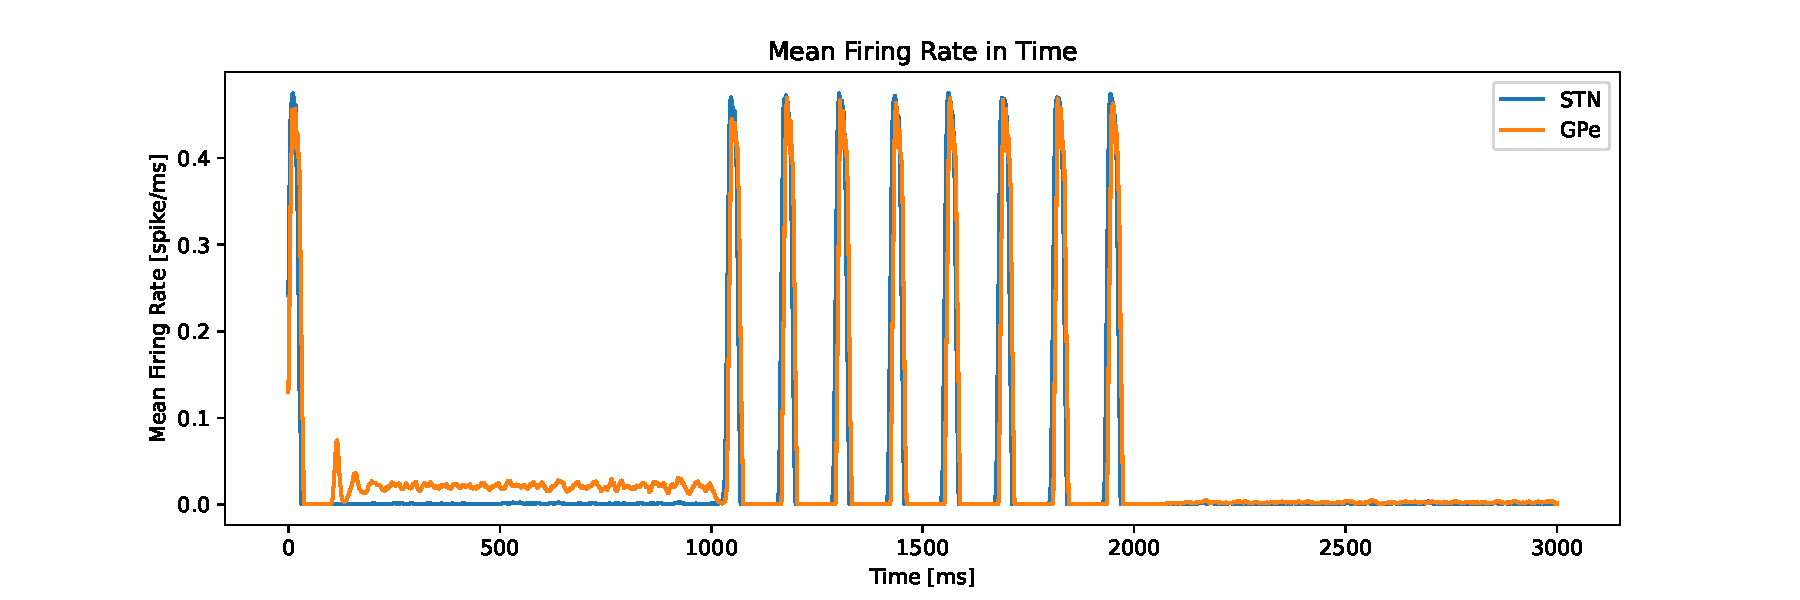
\includegraphics[width=\textwidth]{images/mean_firing_rate.pdf}
    \caption{\textbf{Mean firing rate in different phases:} 
    Mean firing rate of both populations of the neurons computed 
    from the spikes in the last 10 ms interval in each milisecond of the simulation.
    To determine time intervals of the different phases see caption of Figure
    \ref{fig:raster_plot}.}
    \label{fig:firing_rate}
\end{figure}

\begin{figure}[tb]
    \centering
    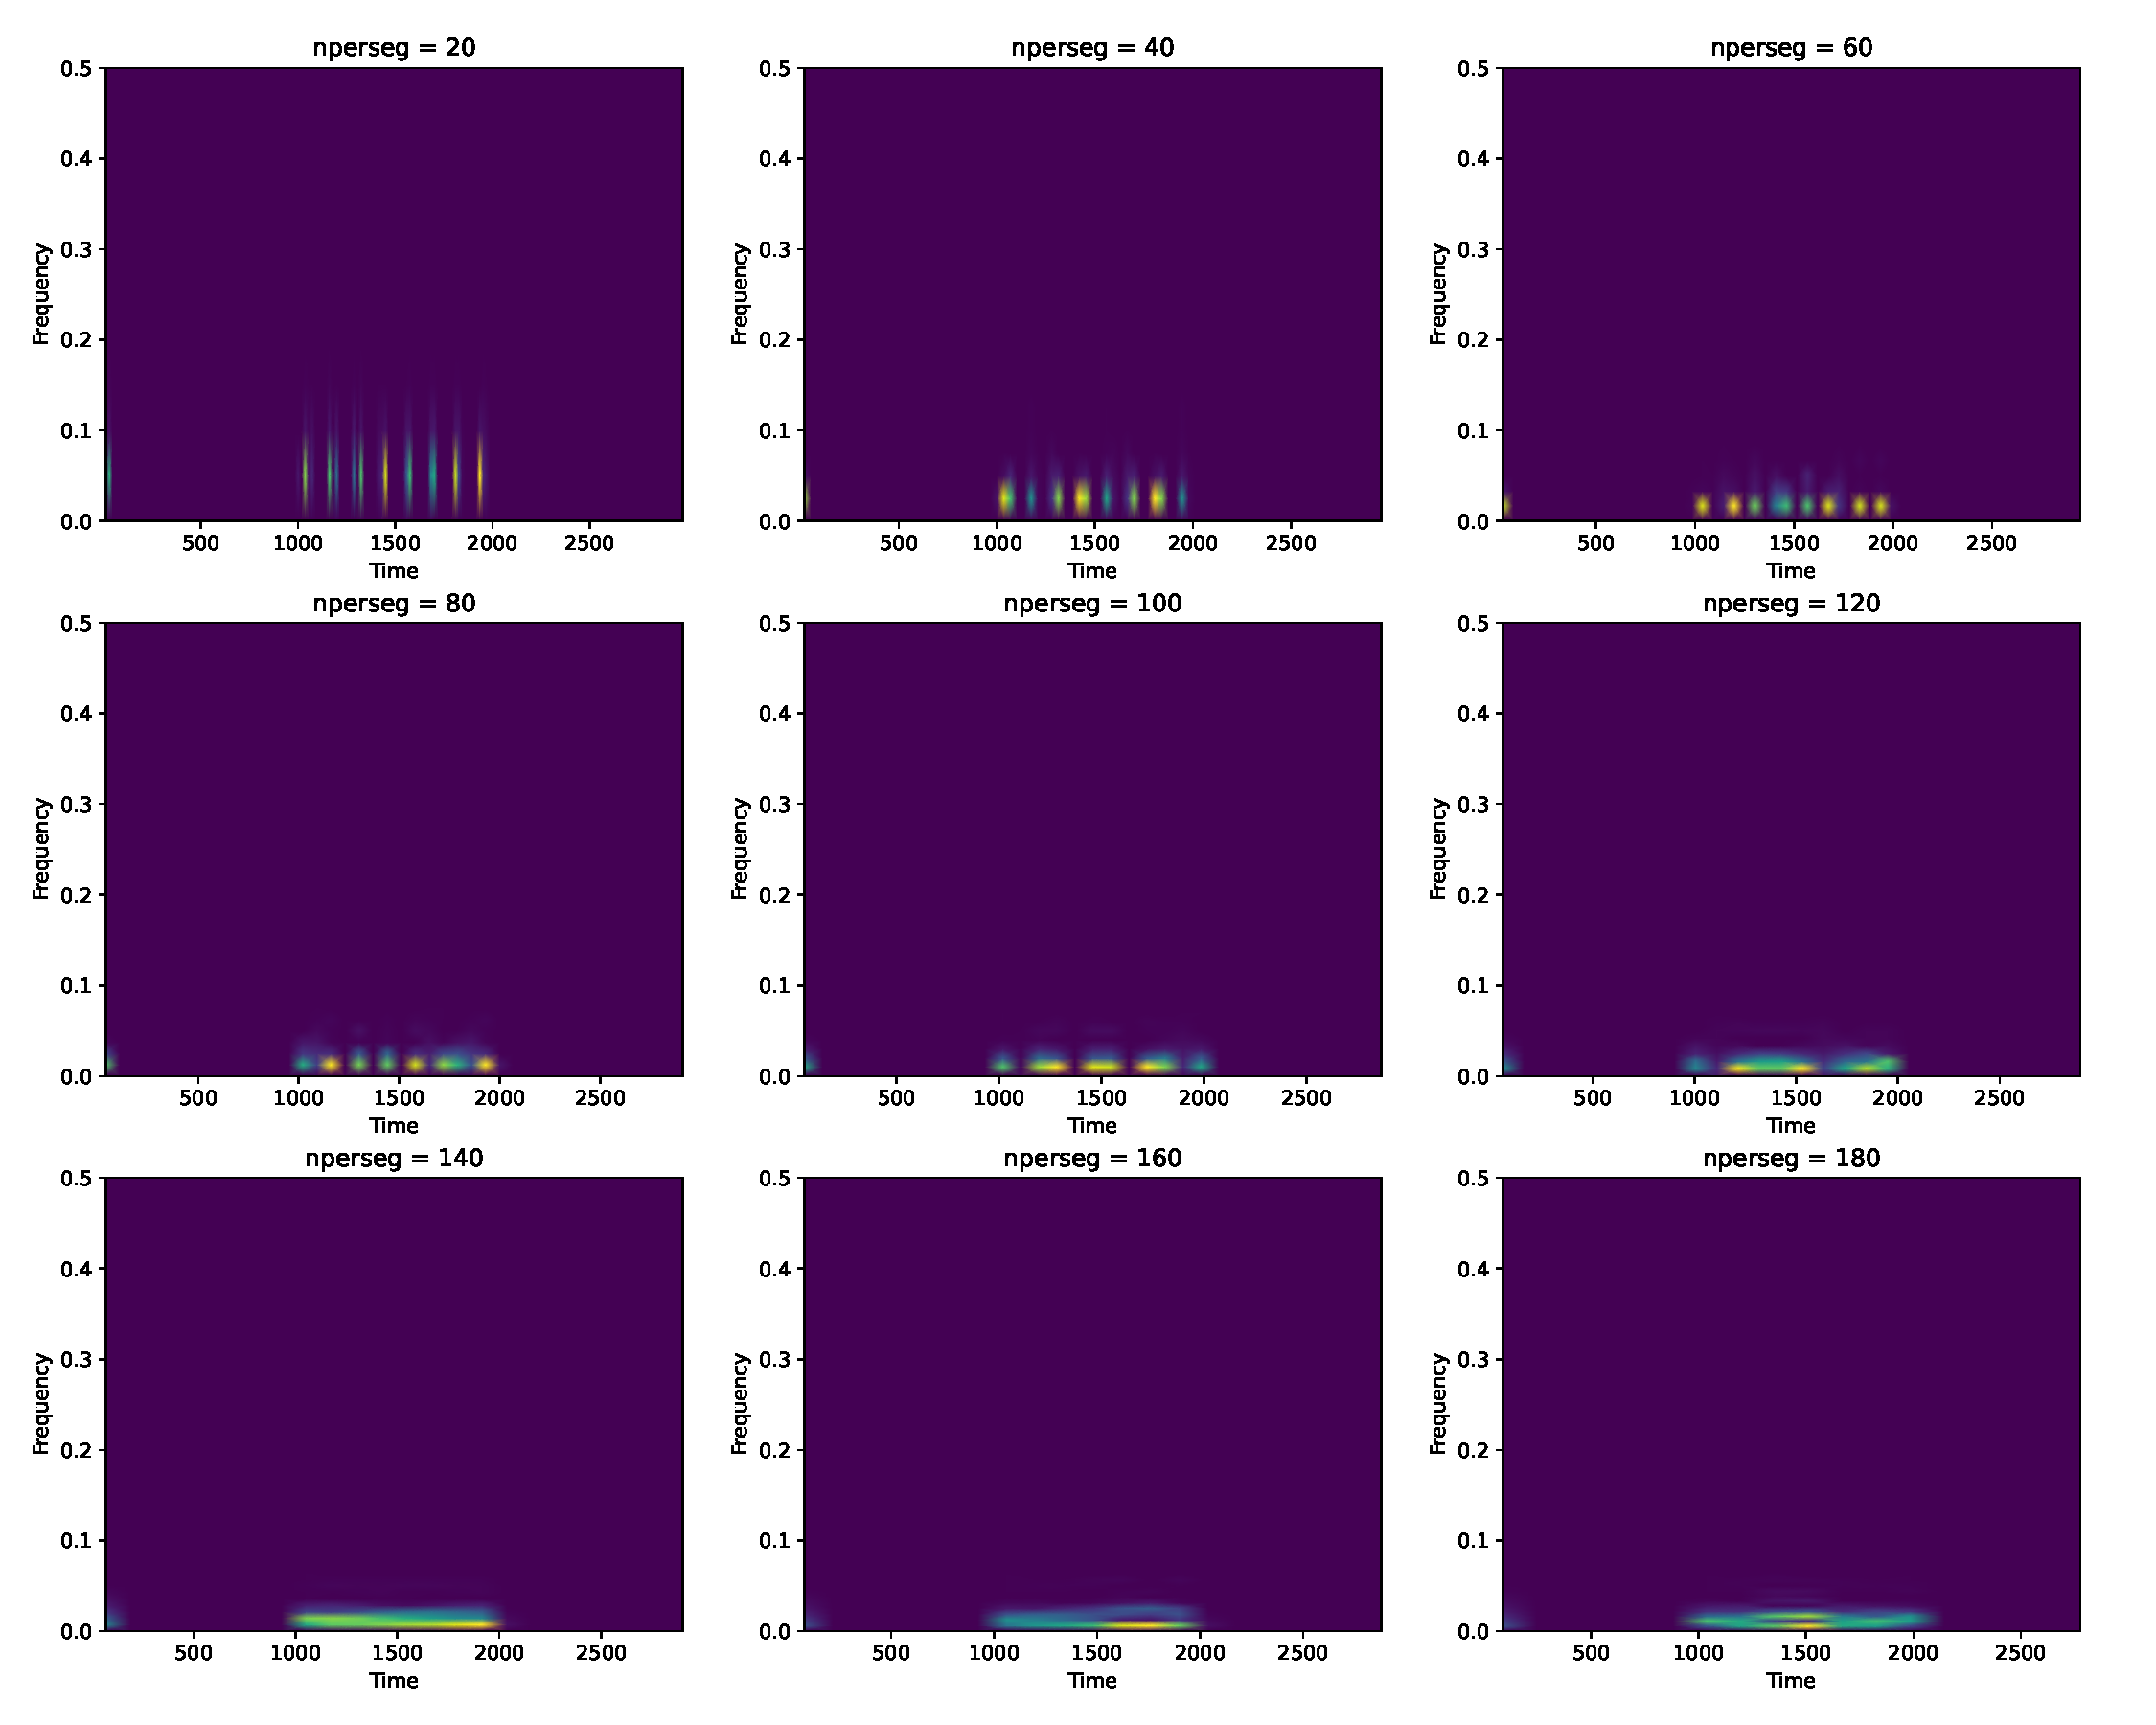
\includegraphics[width=\textwidth]{images/power_spectrum_STN.pdf}
    \caption{\textbf{Power spectrum of STN population:}
    Power spectrum of the STN population for the different time windows to 
    compute the spectrogram (parameter nperseg). 
    To determine time intervals of the different 
    phases see caption of Figure \ref{fig:raster_plot}.}
    \label{fig:power_spectrum_STN}
\end{figure}

\begin{figure}[tb]
    \centering
    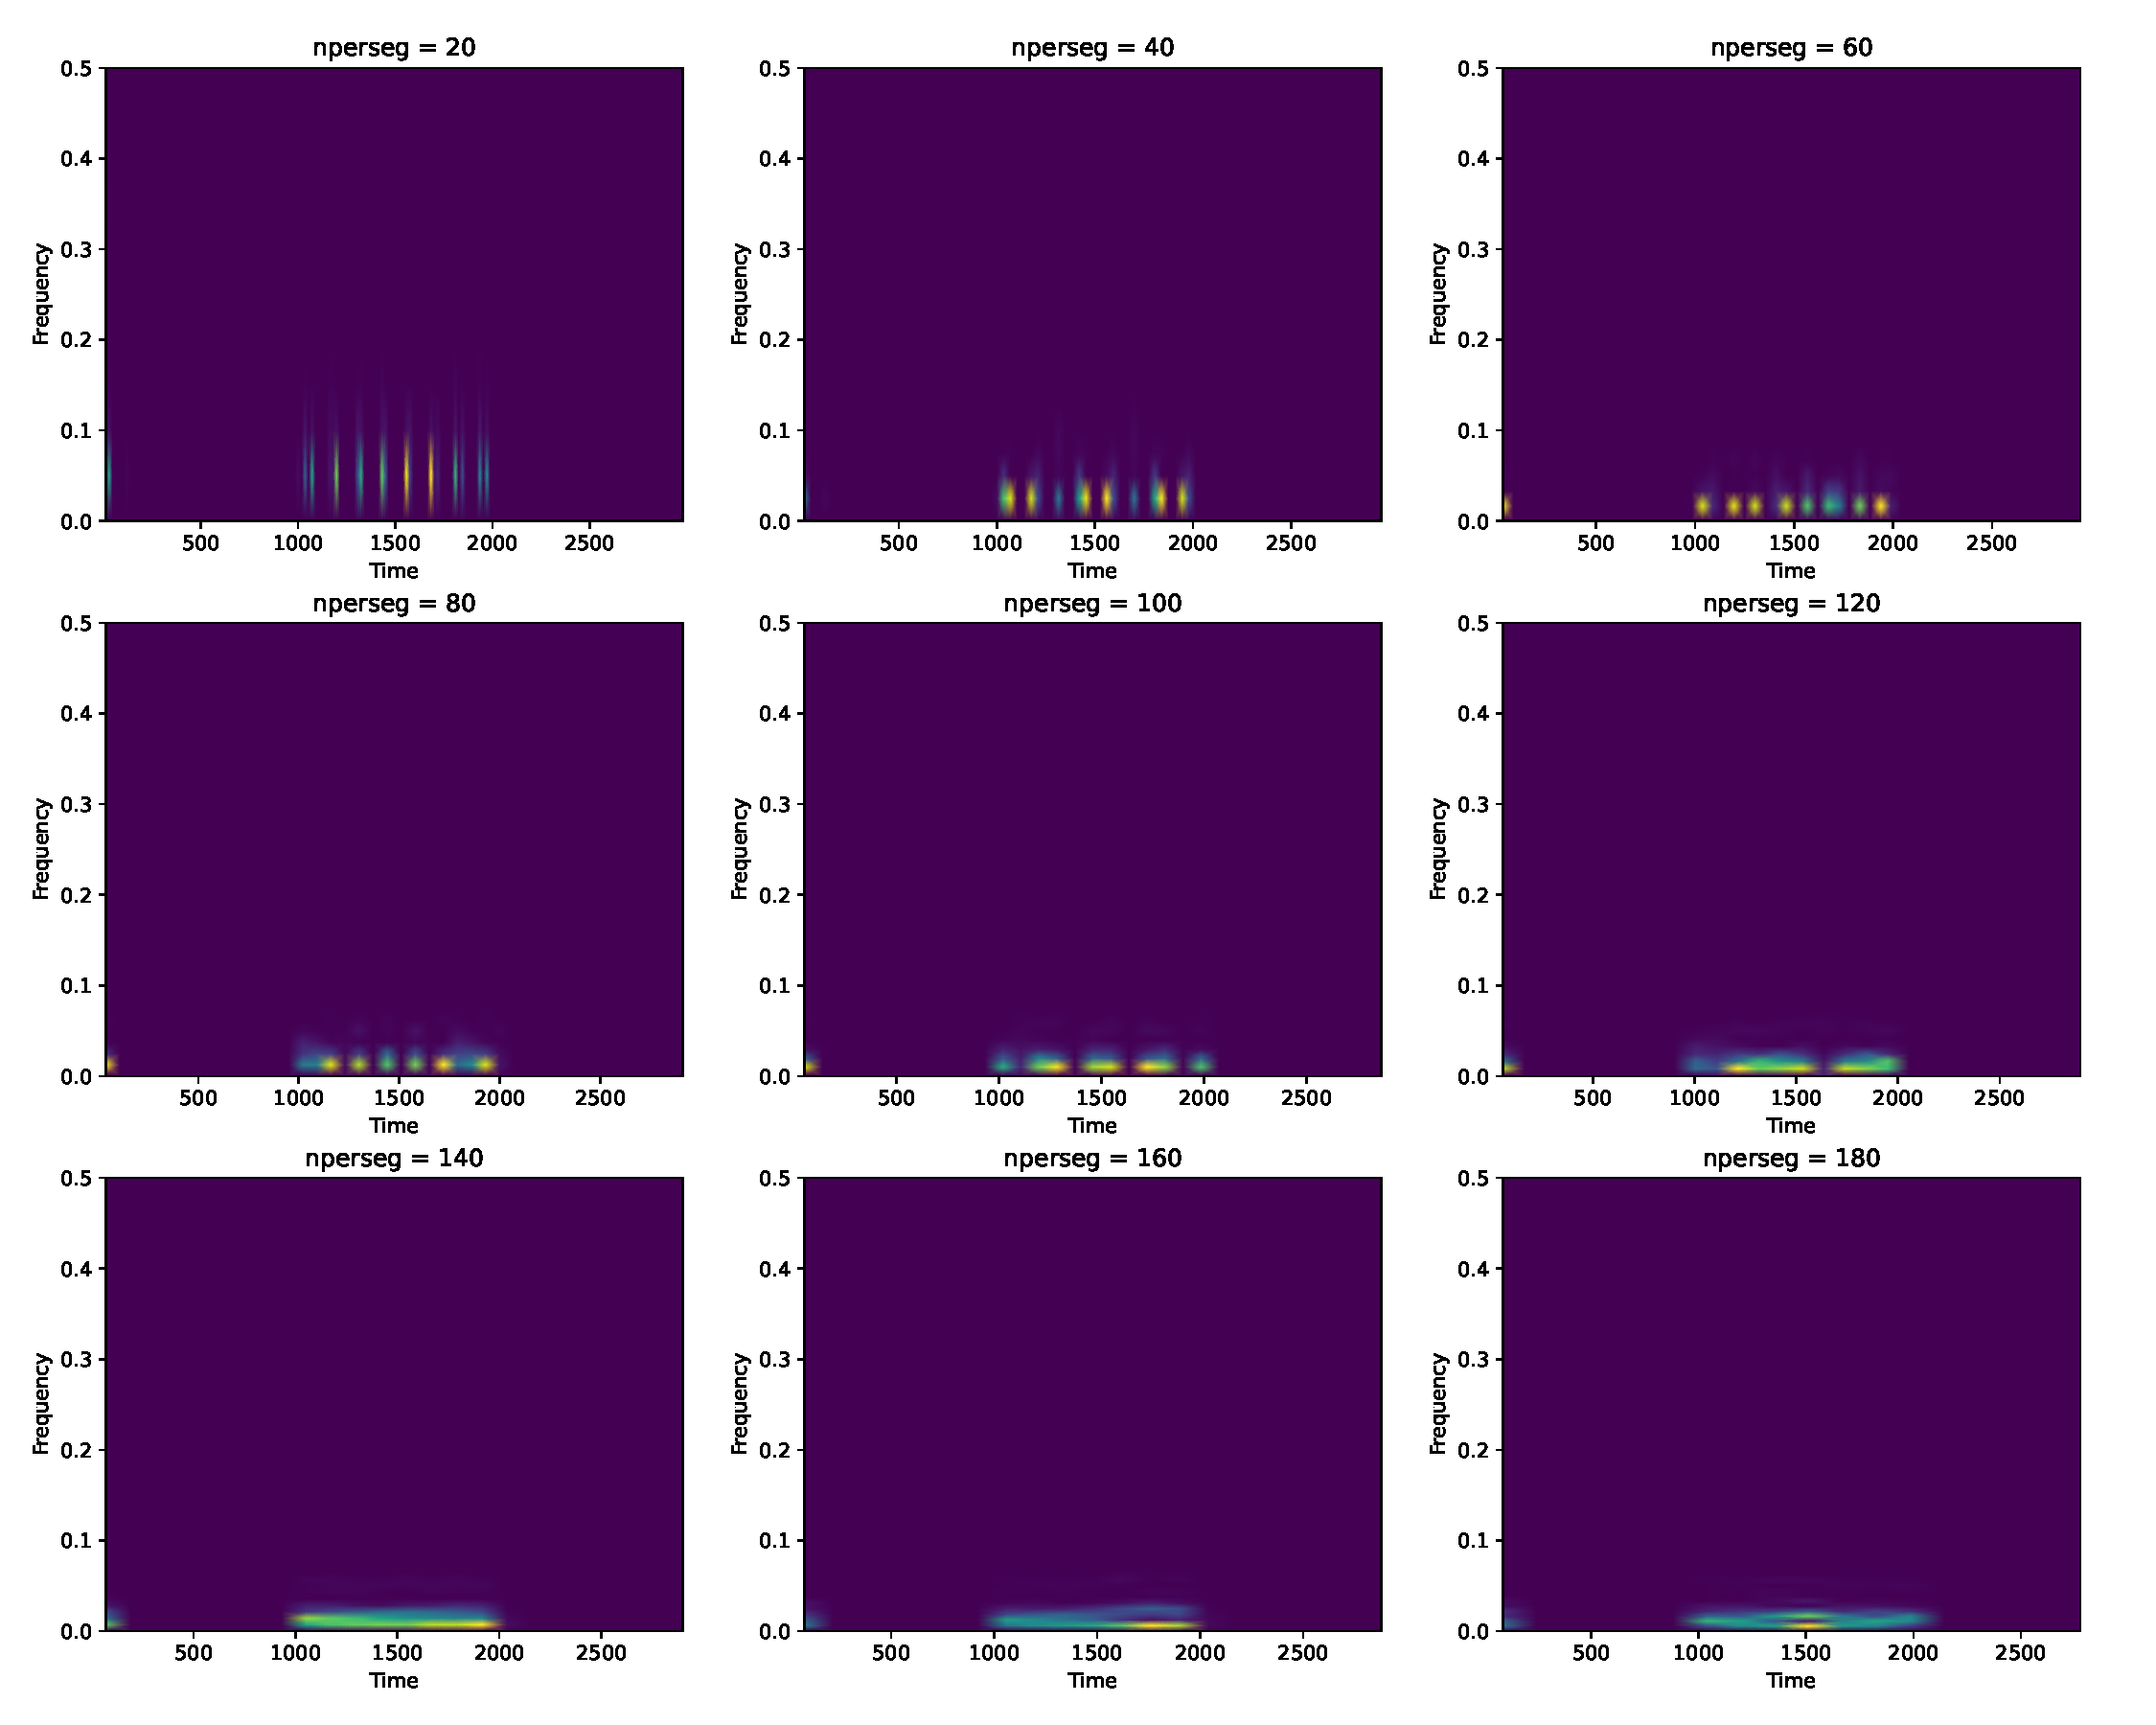
\includegraphics[width=\textwidth]{images/power_spectrum_GPe.pdf}
    \caption{\textbf{Power spectrum of GPe population:} 
    Power spectrum of the GPe population for the different time windows to 
    compute the spectrogram (parameter nperseg). 
    To determine time intervals of the different 
    phases see caption of Figure \ref{fig:raster_plot}.}
    \label{fig:power_spectrum_GPe}
\end{figure}

\begin{figure}[tb]
    \centering
    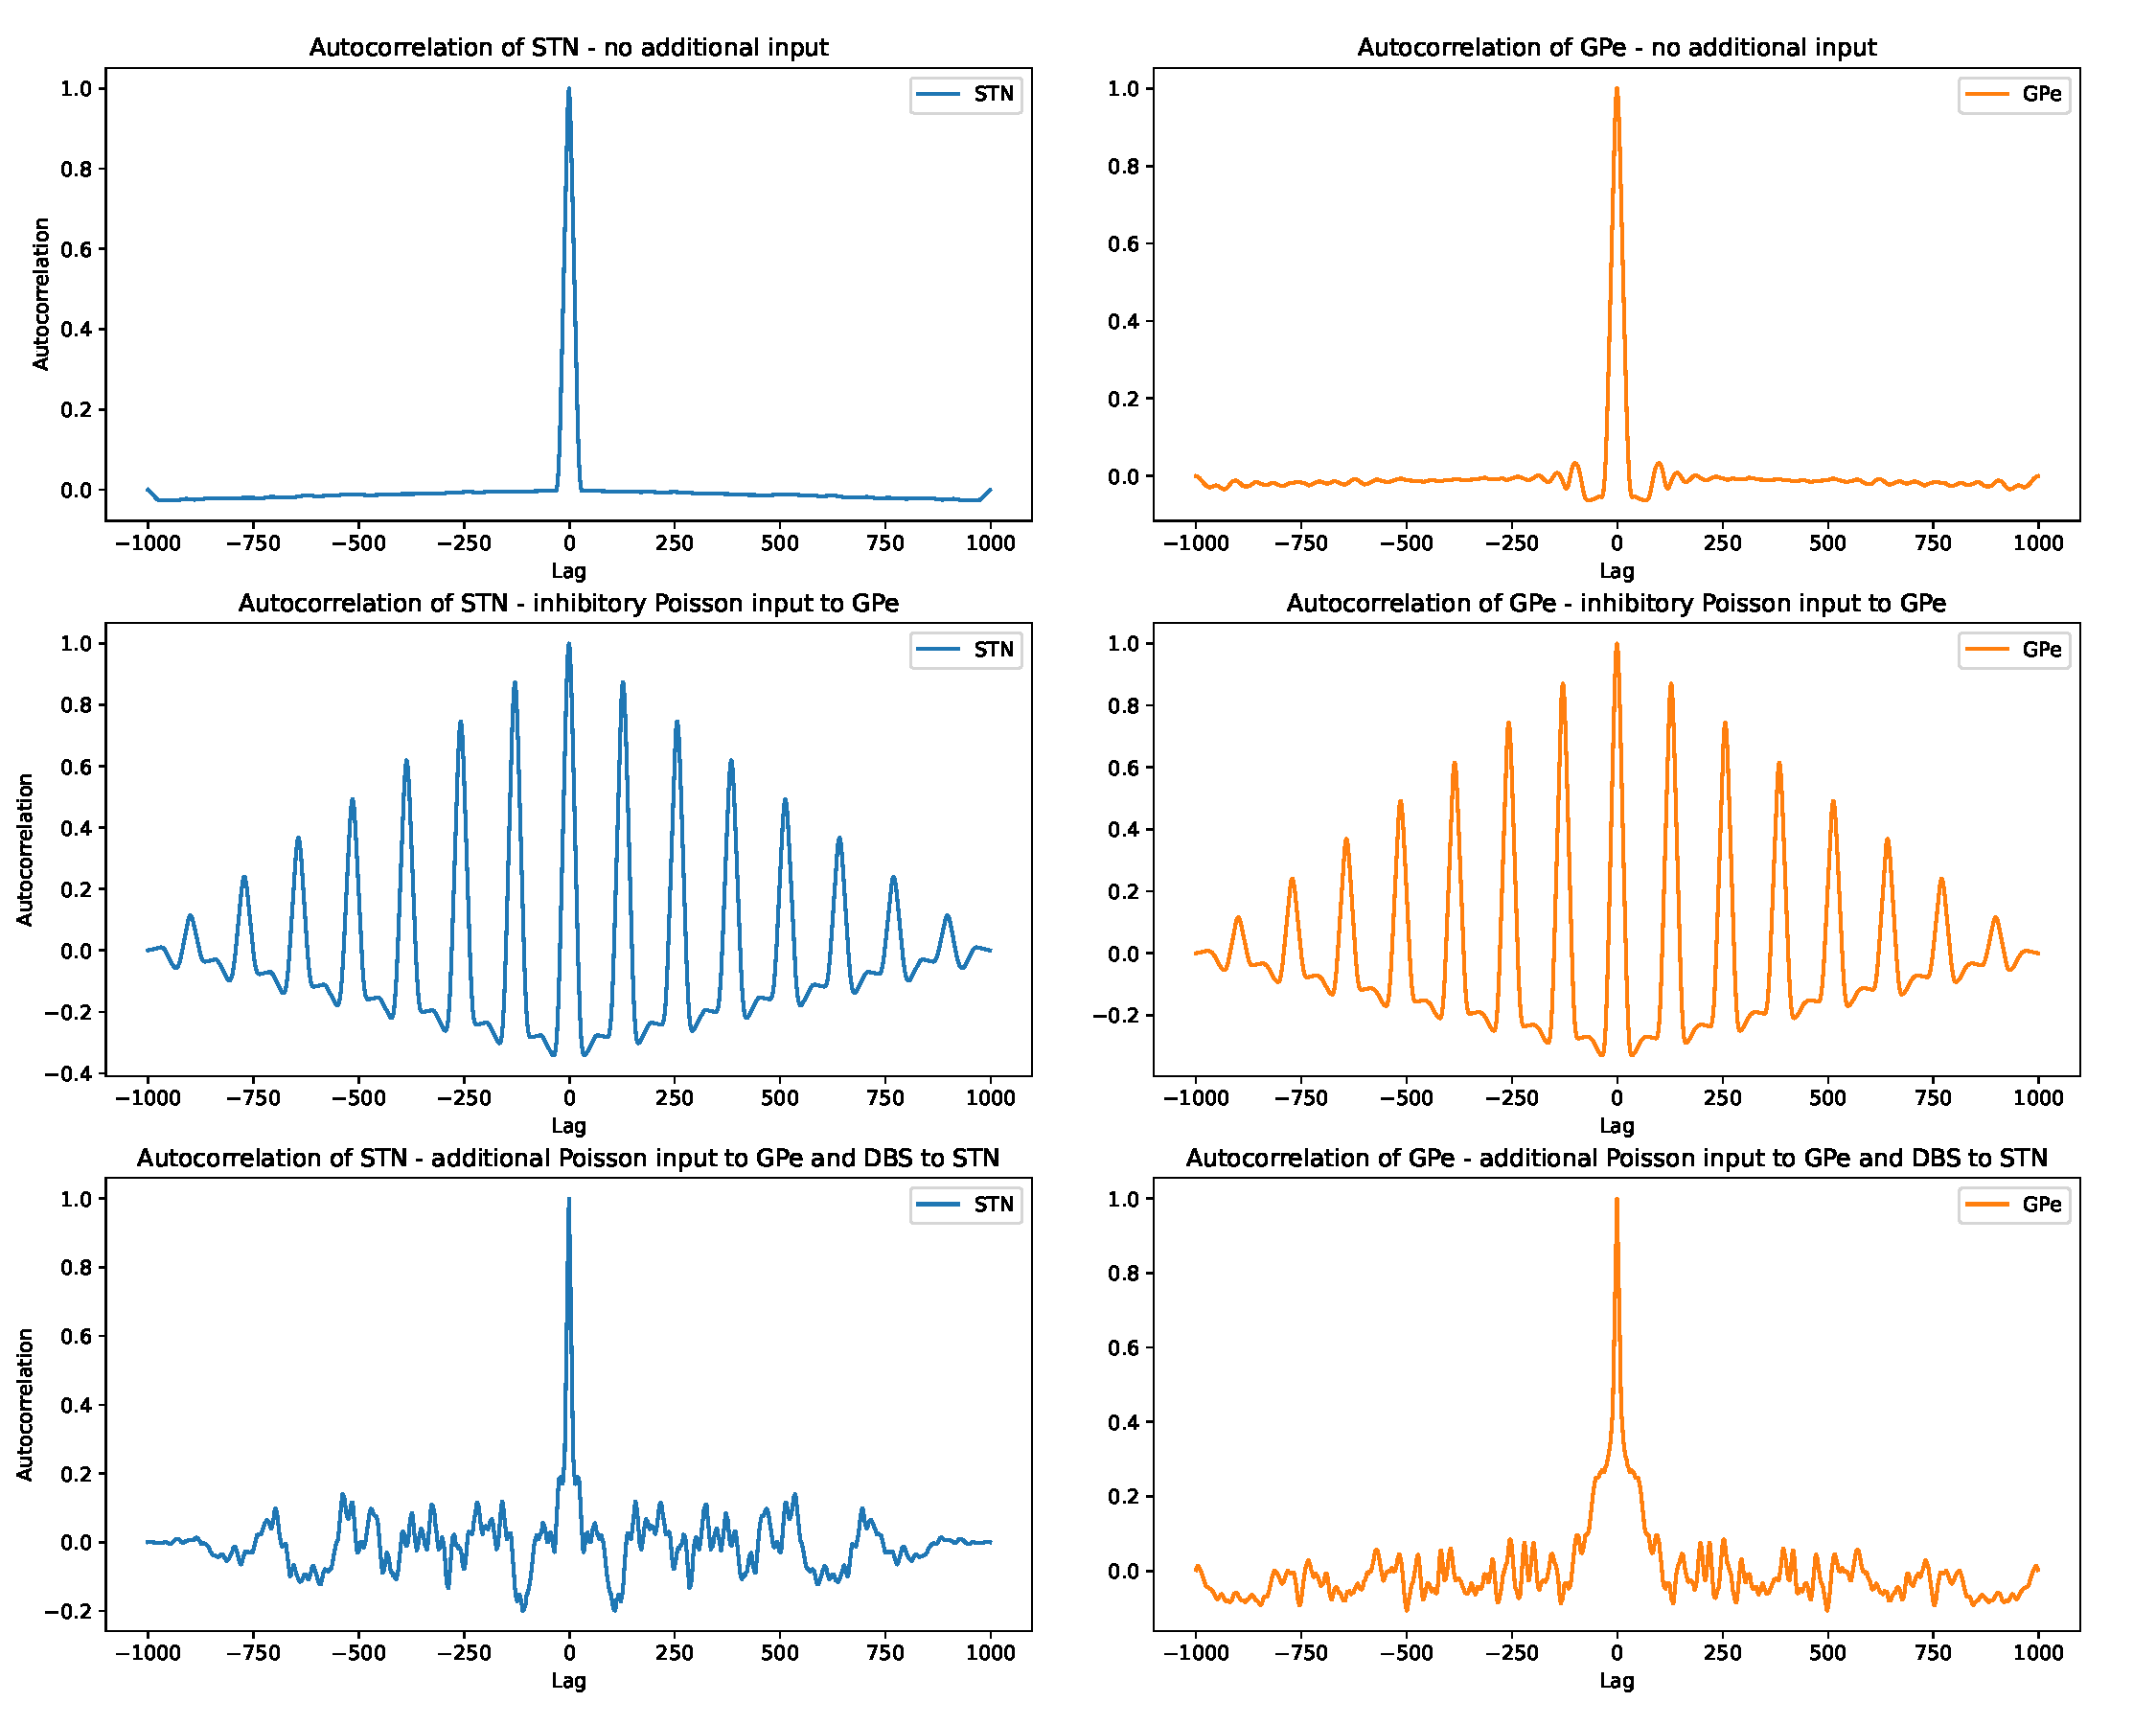
\includegraphics[width=\textwidth]{images/autocorrelation.pdf}
    \caption{\textbf{Autocorrelation in different phases:} 
    Autocorrelation of the firing rate of both populations of STN and GPe neurons in
    all phases of the experiment.}
    \label{fig:autocorrelation}
\end{figure}

\begin{figure}[tb]
    \centering
    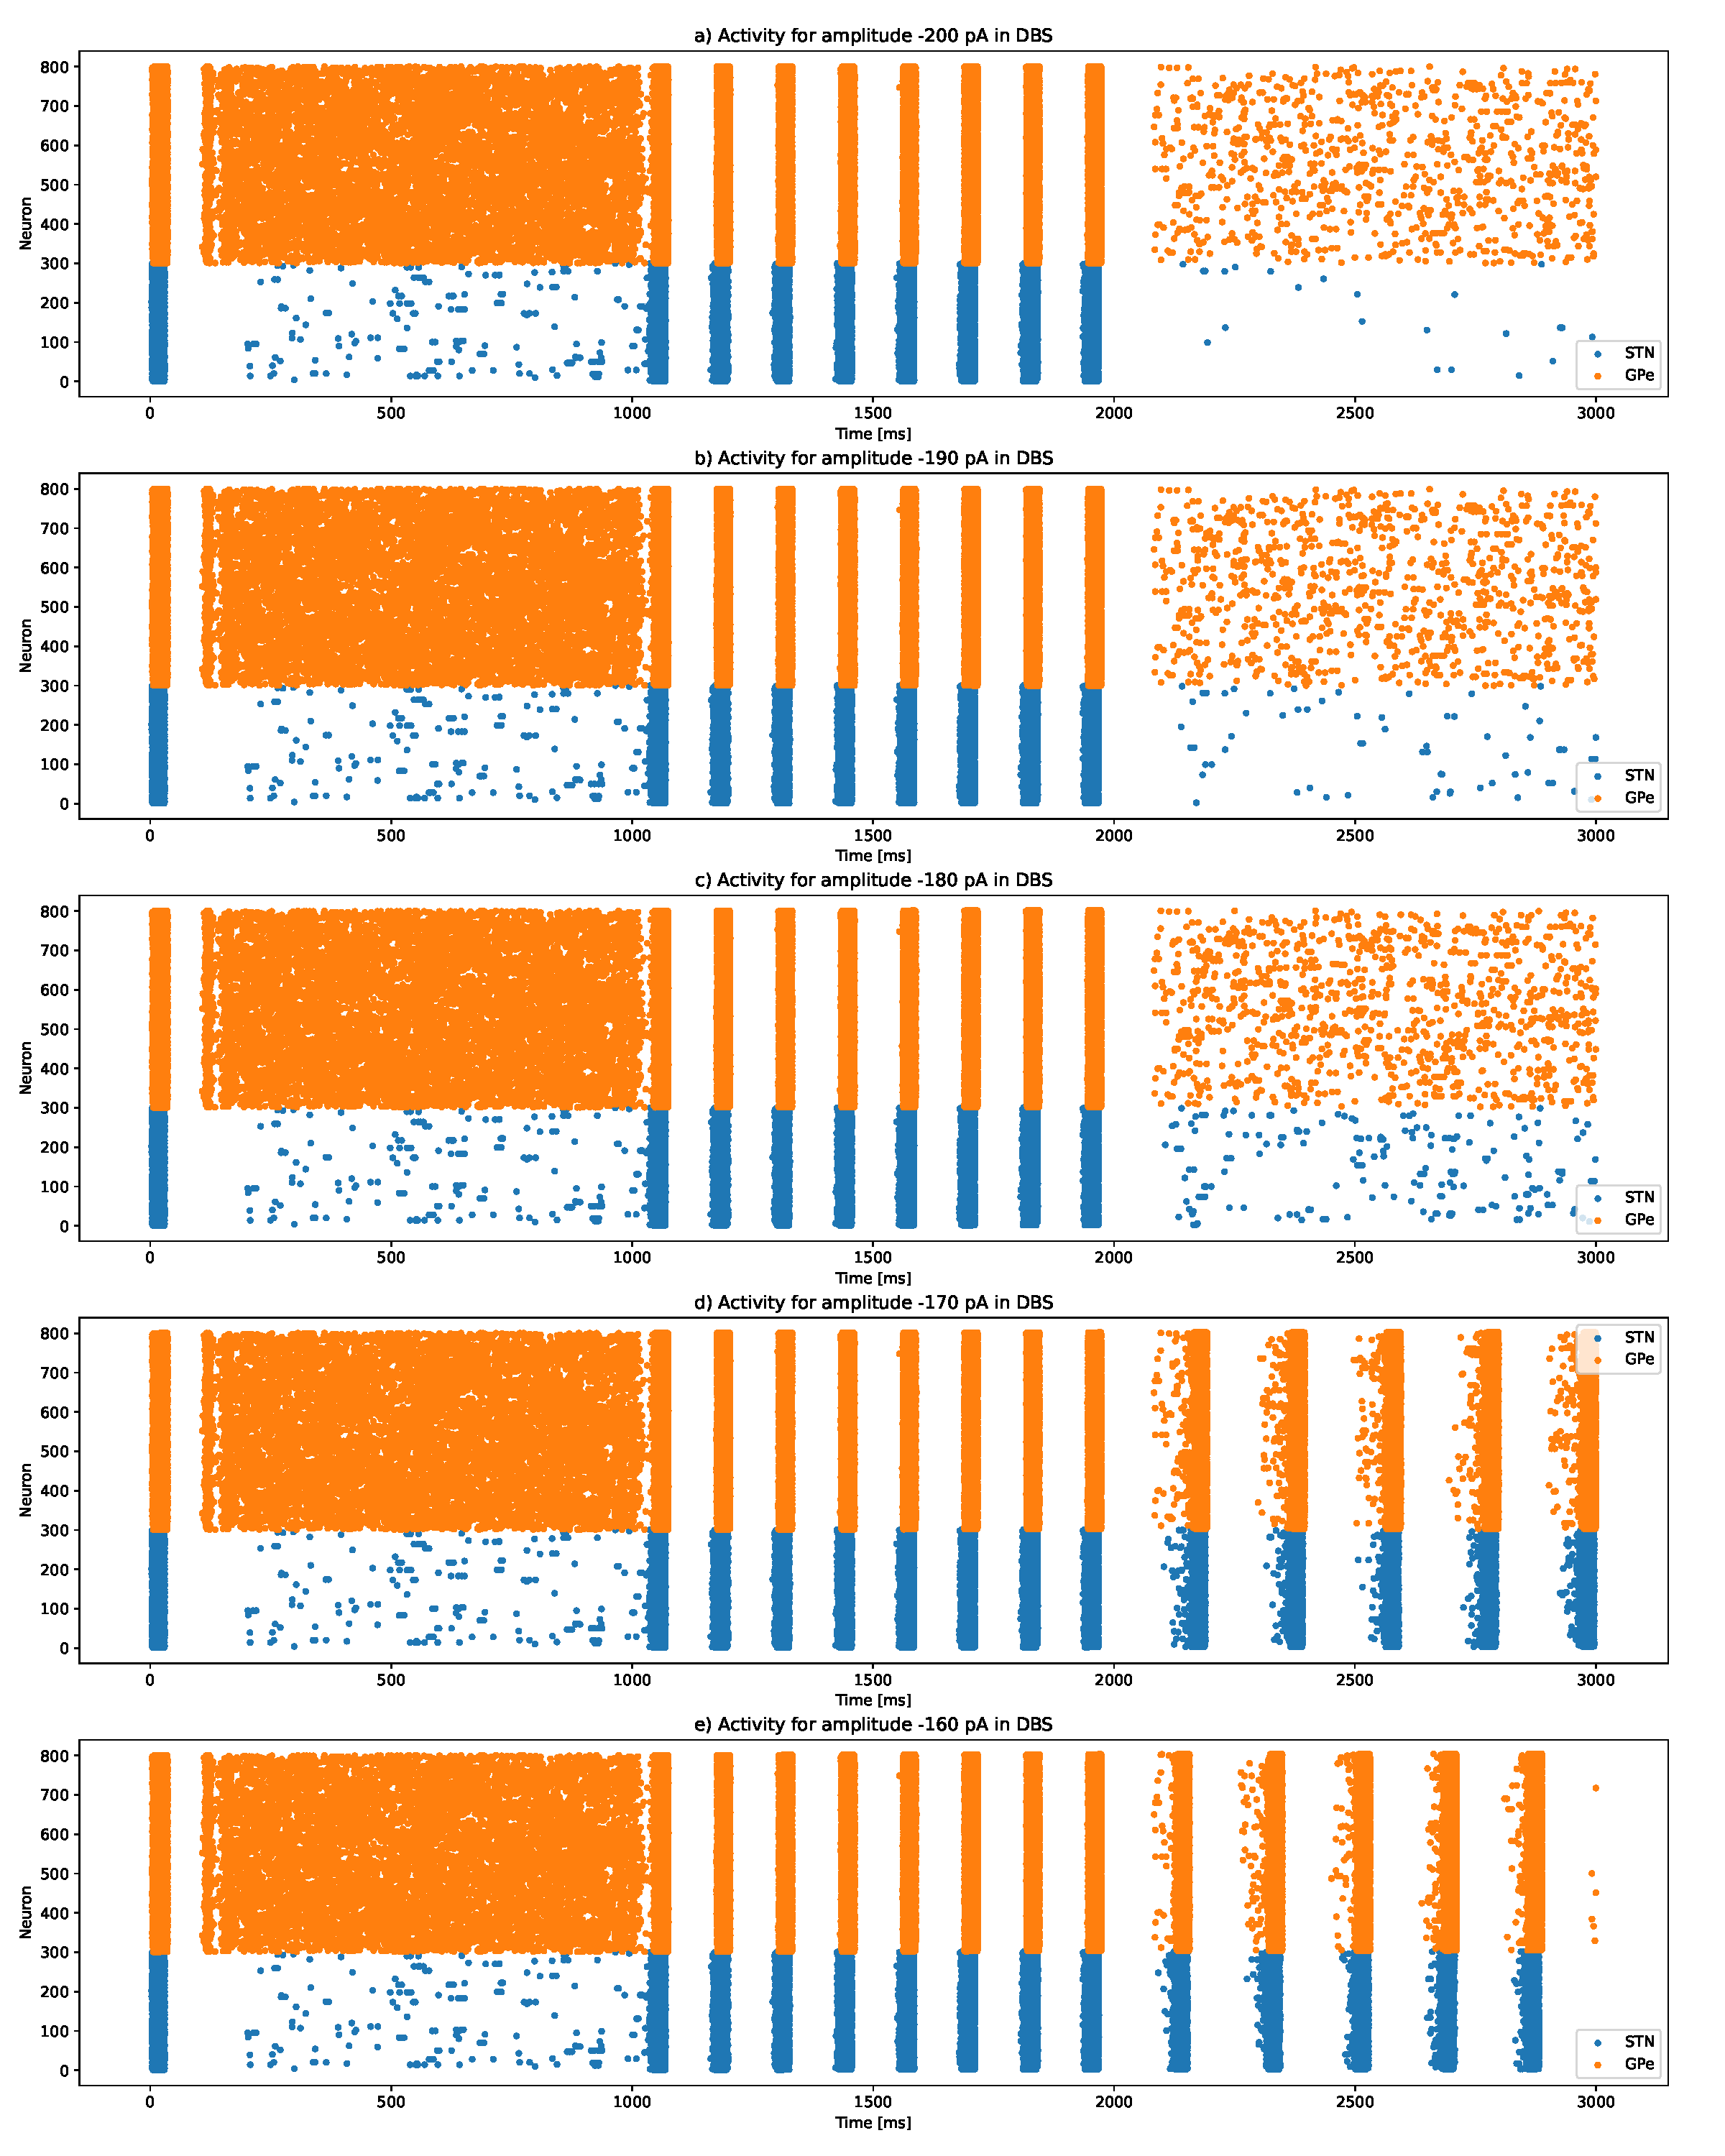
\includegraphics[width=\textwidth]{images/different_dbs_amplitudes.pdf}
    \caption{\textbf{Neuronal activity for different DBS currents (large scale):} 
    Raster plots of neuronal activity in time in 3 different phases of 
    the simulation for different DBS amplitudes
    (overview of the activities for larger scale of currents).
    To determine time intervals of the different phases see caption of Figure
    \ref{fig:raster_plot}.}
    \label{fig:different_DBS}
\end{figure}

\begin{figure}[tb]
    \centering
    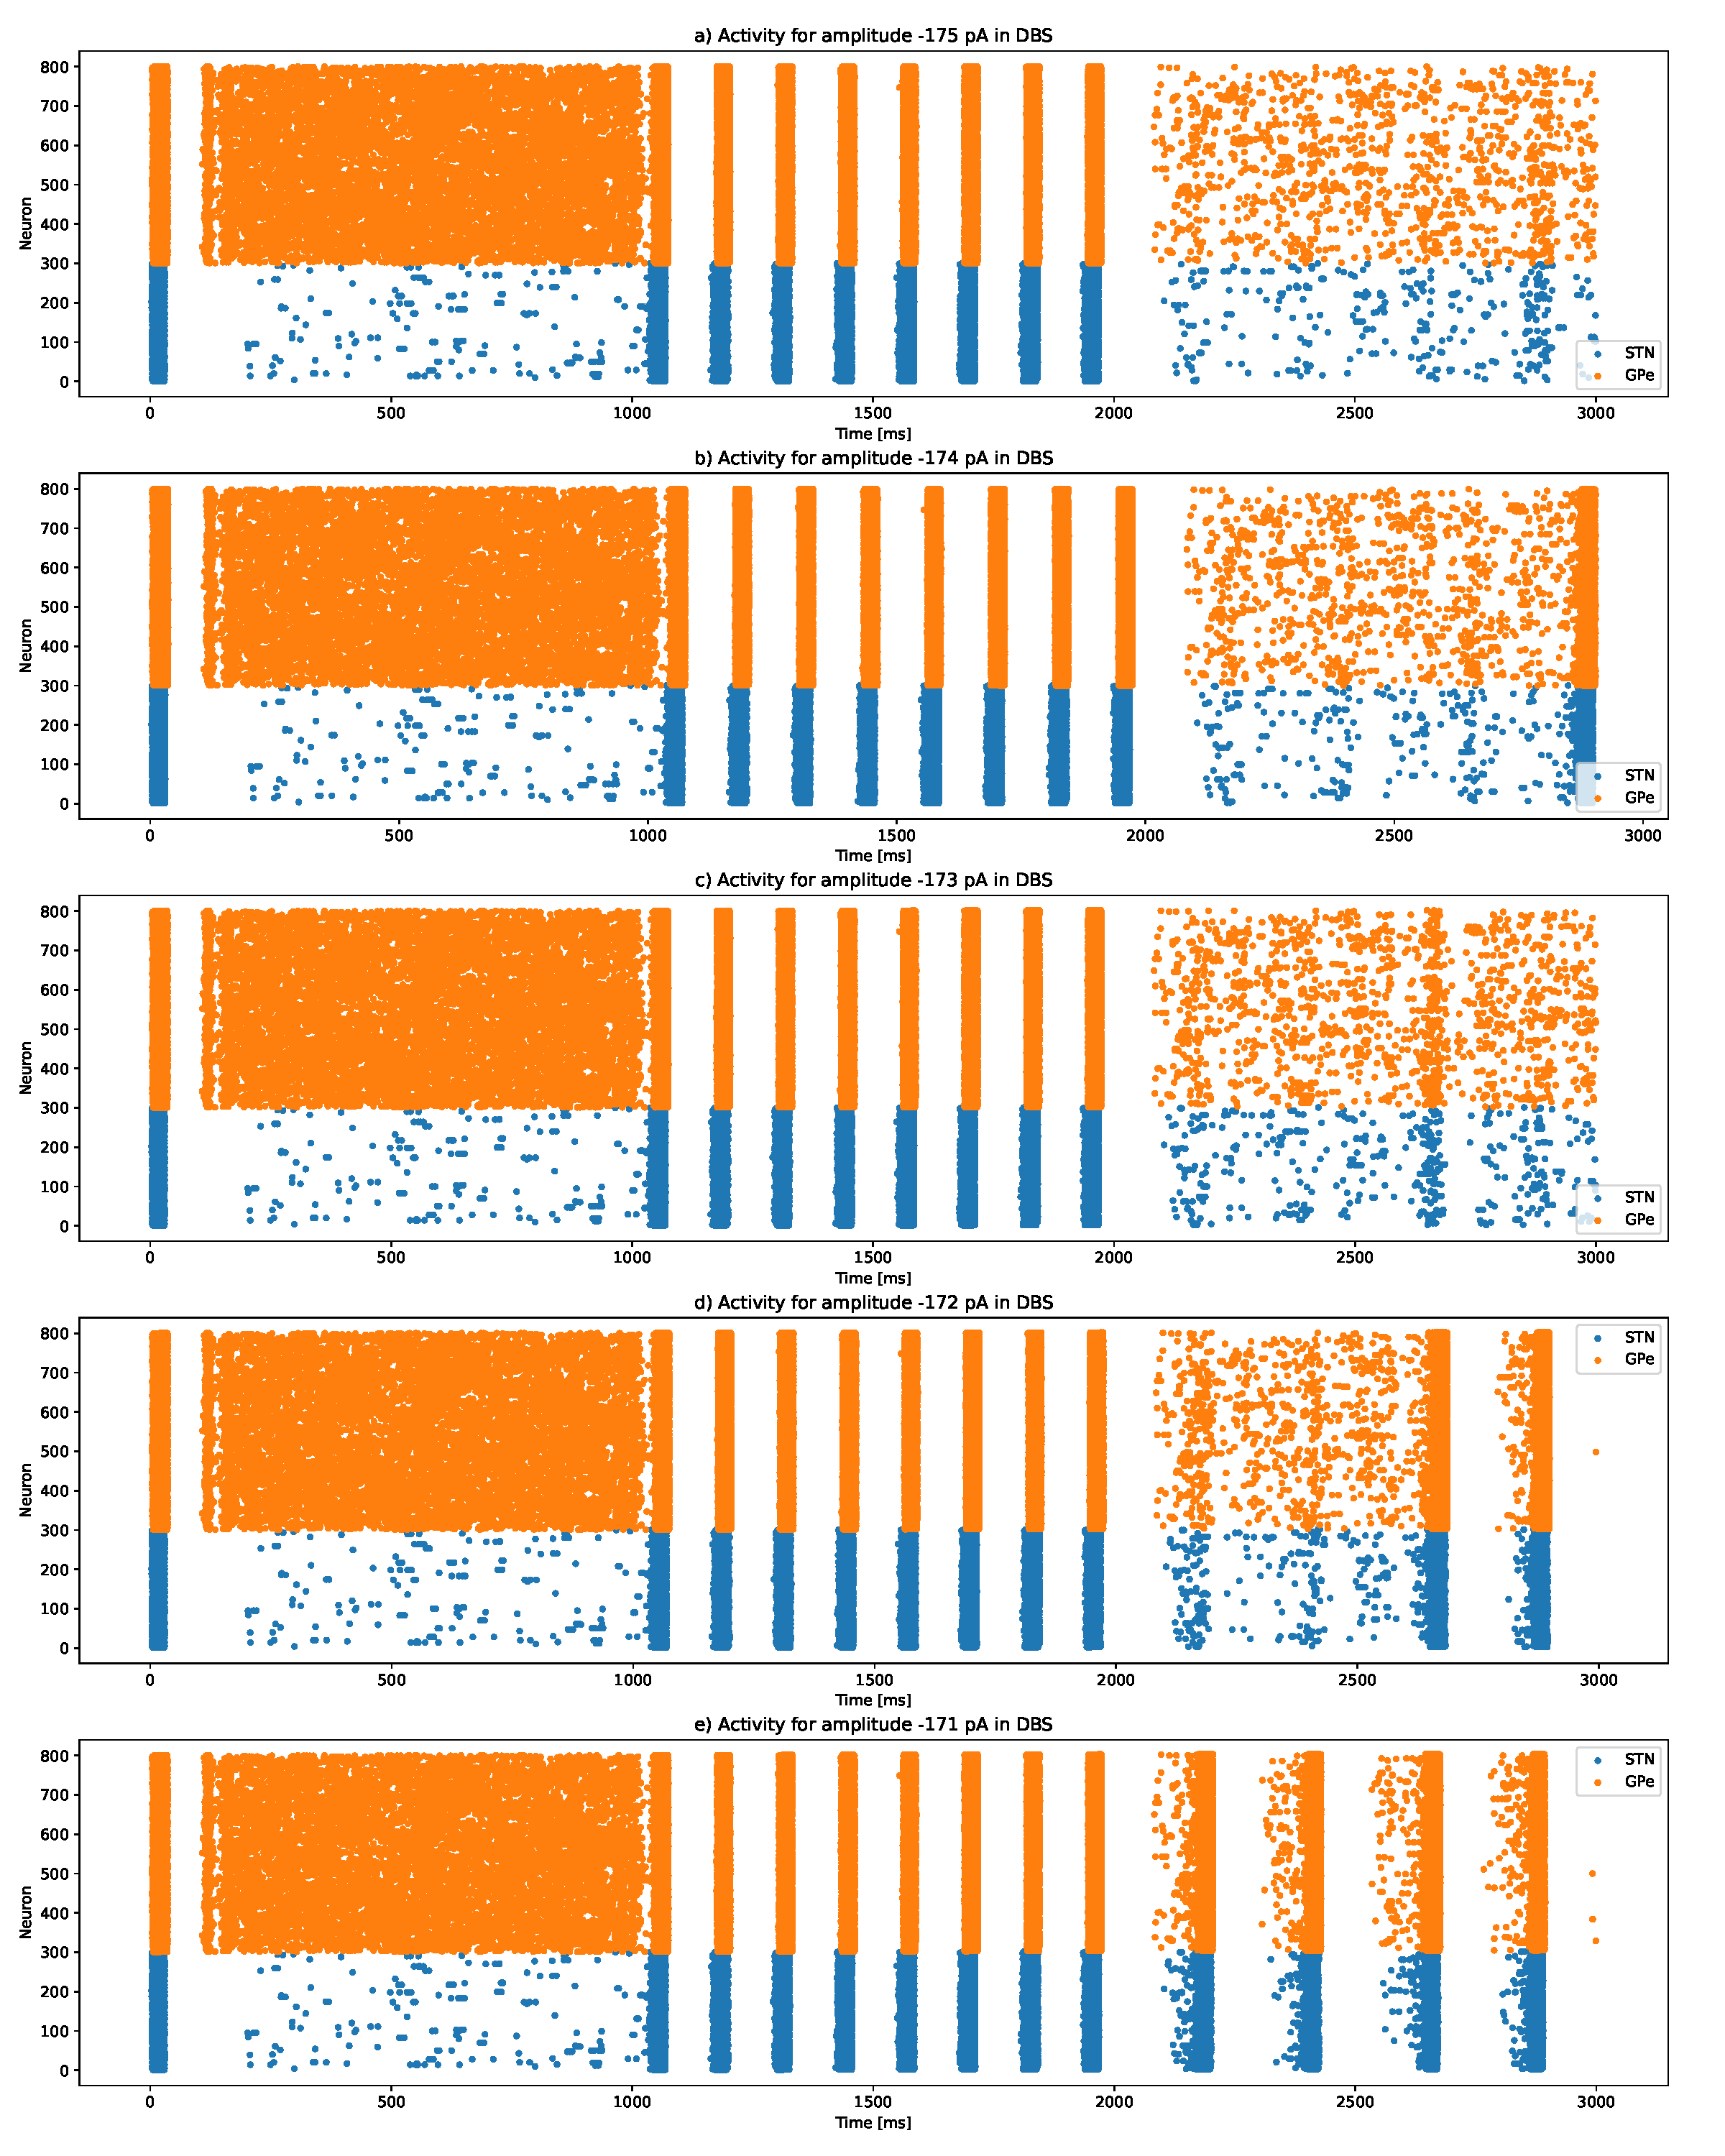
\includegraphics[width=\textwidth]{images/different_dbs_amplitudes_specific.pdf}
    \caption{\textbf{Neuronal activity for different DBS currents (smaller scale):} 
    Raster plots of neuronal activity in time in 3 different phases of 
    the simulation for different DBS amplitudes
    (closer look on the critical interval of activity change).
    To determine time intervals of the different phases see caption of Figure
    \ref{fig:raster_plot}.}
    \label{fig:different_DBS_specific}
\end{figure}


In the first part of the analysis, we plot the raster plot (Figure \ref{fig:raster_plot}) 
of spikes in the simulated populations of neurons in all three conditions. 
We have encountered, that during the first stage (no additional input)
there is high number of 
spikes in GPe randomly distributed in time (when we ignore first milliseconds of the 
simulation that are influenced by the start of the simulation). Spikes of the 
STN neurons are also randomly distributed in time, but the count of them is 
significantly smaller than of GPe neurons. These properties correspond 
with the healthy state of the brain. 
After adding inhibitory
input to GPe, we can see significant change of the distribution of spikes. In this time
interval, the spikes of both populations of neurons are coupled in small time intervals
that occur periodically. We can see small shift in spikes of GPe in comparision to STN.
Reason of this could be the excitation of the GPe neurons with the STN input and following
inhibition of all neurons with the GPe input. This stage of the simulation corrensponds
with the slow oscillations in PD. 
Lastly, after DBS, we see similar behavior of the neurons as in the healthy state. 
Although, there is a significant change in the number of 
spikes of GPe neurons in comparision to the first part of the simulation. This is probably 
the consequence of inhibition of GPe. Because, the spikes look randomly distributed, we
conclude that the DBS depleted the oscillations. These results correspond with 
improvement of the state of pacients with PD after applying DBS.

We then analyse other parameters of the model to make sure our assumption is true.
We plot mean firing rate through the whole simulation (Figure \ref{fig:firing_rate}).
We compute mean firing rate (spikes in ms normalized with the size of the population) in 
each second using last 10 ms intervals of the simulation. After ploting, we can see properties
that support our statemens mentioned above. We can see that mean firing rate of 
GPe population is slightly larger in stage without additional input in comparision 
to DBS state which corrensponds to smaller number of spikes in DBS state. Also, we can
see periodic rise and decline of mean firing rate in GPe inhibition state, which
corrensponds to oscillations of the neural firing.

Similarly, in the spectrograms of mean firing rates 
(Figure \ref{fig:power_spectrum_STN} and \ref{fig:power_spectrum_GPe}), 
we can see that the power spectrum in GPe inhibition
state is biased towards specific frequencies, which can be the indicator of oscillations.
In comparision to the other two phases (no input and DBS), where the power spectrum is 
almost uniform, which indicates the randomness of the firing rate in time.

Another confirmation of our results are the plots of the autocorrelation 
(Figure \ref{fig:autocorrelation}). We can see that in the
no additional input state the correlation almost instantly declines to 0 with time shift, 
which indicates the independence of the spikes in time. In the DBS stage, there are 
similarities with no input stage. Though, we can see small correlations through the whole
range of time shifts. This indicates, that the spikes are probably slightly dependent
between themselves. In contrast, in the variant with only GPe inhibition, we can see 
significant oscillation of autocorrelation value in time shift, 
which indicates that the spikes probably are not 
independent. This property might be caused by the periodic oscillation of the spikes.
There is no significant difference beteween STN and GPe neurons. GPe neurons look
slightly more correlated in time in no input stage. This fact might be caused by 
higher number of neurons. Furthermore, in DBS stage the absolute value of correlation 
is slightly smaller in GPe than in STN. This property is probably the result of 
GPe inhibition in this stage.

Lastly, we research how sensitive is the effect to changes in the DBS
amplitude. We run the simulations for different amplitudes of DBS. First, we
perform large scale overview of the dependence on the DBS amplitude 
(Figure \ref{fig:different_DBS}). In this experiment, we choose currents
in range from -200 pA to -160 pA with 10 pA steps. We find out that for smaller 
values than default current -180 pA the number of spikes in STN neurons declines
(expected, because in DBS we inhibit the STN neurons). Additionaly, when we
increase the current to -170 pA and -160 pA, we see significant change 
of the neuron behavior in both variants towards the oscillation. In addition,
we can see that the stripes of the neuronal
spikes are getting narrower with the higher values of the input current in DBS.

We have seen that the most interesting change of the effect happens around 
the current -170 pA. We perform another simulations for amplitudes in range 
from -175 pA to -171 pA with 1 pA steps 
(Figure \ref{fig:different_DBS_specific}). We can see that there is a hint of
the oscillations in all variants. But, the most significant change of the behavior
of the spiking happens in range -173 pA to -171 pA. In this interval, we can see
almost complete trasformation from "random" spiking  towards periodic spiking
in both populations of the neurons (oscillations). In the end, we mention that the periodic behavior
of the neurons in the DBS which uses higher current than default -180 pA is 
different from the periodical effect in the variant without DBS (only inhibiton of GPe).
The spikes in the DBS are distributed in wider stripes than in only inhibition variant.

After modeling simplified neural model in the NEST simulator, we have encountered that
our model performed fairly well in case of reproducing the results from the work of 
Kumar et al. mentioned in the project description.

\end{document}